\newpage
\section{Mapeo de características}

\subsection{Introducción}
Utilizando el mismo dataset de Bag of Words (BOW) del ejercicio anterior debemos construir un modelo de mapeo de características auto-organizado que clasifique automáticamente los 
documentos en un arreglo de dos dimensiones. Este problema será resuelto utilizando Kohonen.

Kohonen:
\begin{itemize}
	\item Propone un orden topológico y un modelo competitivo
	\item Función de transferencia 
				\begin{align*}
					O_{i}=f(\varepsilon, W_{i}) donde W_{i}=(w_{i1}, ..., w_{in}) \in \mathbb{R}_{n}
				\end{align*}
	
	\item PRINCIPIO DE ADAPTACIÓN: Consiste en detectar la unidad cuyos parámetros sean más parecidos a la entrada $\varepsilon$.
		\begin{itemize}
			\item Establece un orden topológico y solo se cambian los parámetros de la unidad seleccionada y los de sus vecinas.
			\item El cambio es en dirección de incrementar la sililaridad entre $W_{i}$ y $\varepsilon$.
			\item La magnitud del cambio debe garantizar estabilidad asintótica.
		\end{itemize}
		Estas tres cosas hacen que la función de densidad de probabilidades de $W_{i}$ tienda a aproximar la densidad $P(\varepsilon)$.
	\item MAPAS DE KOHONEN: Es una propuesta de implementación la cual define:
		\begin{itemize}
			\item Que la unidad seleccionada en tiempo $t$ será $c$ tal que:
				\begin{align*}
					||\varepsilon(t) - W_{c}(t)|| = min\{\varepsilon(t) - W_{i}(t)\}
				\end{align*}
			
			\item Se establece una topología de entrada a partir de establecer funciones de vecindad, esto fuerza a que los pesos no crezcan de una forma desmedida respecto de los 
			pesos de las unidades vecinas. Esto hace que los entornos sean amplios al principio pero pequeños al final, hasta limitarse solo a la unidad seleccionada.
				
			\item REGLA DE KOHONEN: Actualización de los $W_{i}$.
					\begin{align*}
					 W_{i}(t+1) &=  \begin{cases}
										W_{i}(t) + \alpha(t) [ \varepsilon(t) - W_{i}(t) ] & i \in N_{c} \\
										W_{i}(t)                                           & i \not \in N_{c}  
									\end{cases} \\
					\end{align*}
			\item $\eta(t)$ es el coeficiente de aprendizaje dinámico, decreciente en el tiempo.
				\begin{align*}
					\Delta W_{ij} = \alpha(t) [ \varepsilon(t) - W_{i}(t) ]
				\end{align*}
				\begin{align*}
					\alpha(t) = \eta \Lambda(i,c)
				\end{align*}
				\begin{align*}
					\Lambda(i,c) = \begin{cases}
										1 & i = c \\
										decrece a mayor distancia entre i y c 
									\end{cases} \\
				\end{align*}
		\end{itemize}
	\item TEOREMA DE KOHONEN: Con probabilidad 1 los $W_{i}$ se ordenan de forma ascendientes o descendientes cuando $t \to
		\infty$ si $\alpha(t) \to 0$ con suficiente lentitud.
\end{itemize}

\subsection{Modelo}
Al igual que en el ejercicio anterior, el conjunto de datos contiene 900 documentos con 856 descripciones de texto correspondientes a compañías Brasileñas clasificadas en nueve categorías distintas.

En primer lugar sabemos que la red a entrenar tendrá un aprendizaje no supervisado, ya que no sabemos el resultado al quequeremos llegar.

Definimos nuestro modelo como:

\begin{figure}[ht!]
	\centering
	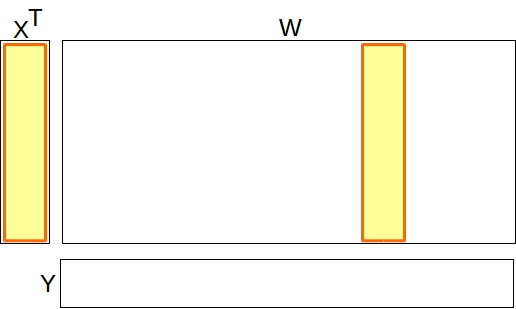
\includegraphics[width=0.7\linewidth]{img/parte2-comparacion.jpg}
	\caption{Comparación}
	\label{comparacion}
\end{figure}

$X$ es el vector de entrada. $X \in \mathbb{R}^{856x1}$ \\

$W$ es diccionario de salida de nuestra red, cuyas claves son pares $(i,j)$ y los significados son vectores en $\mathbb{R}^{856}$.\\

$Y$ es la matriz resultado. $Y \in \mathbb{R}^{M}$ con $M = M_{1} . M_{2}$ que es el tamaño del layout, el cual será definido más adelante.\\

\subsection{Implementación}

\subsubsection{Prepocesamiento de datos}
Al igual que el ejercicio anterior, preprocesamos el dataset centrando los datos en el 0. Calculamos la media de las frecuencias de cada palabra (posición del vector) y le restamosa cada una de ellas. De esta forma, la media de cada columna del dataset resultante es 0 y los datos quedan distribuidos alrededor del 0. En este caso, los datos no se normalizan ya que quedarían todas las dimensiones con la misma varianza y la red no podría aprender correctamente.

\subsubsection{Pseudocódigo}

Inicializamos la matriz de pesos con valores random $\in[-1/2, 1/2]$.

Aclaramos que utilizamos un 70$\%$ del dataset para entrenamiento y el 30$\%$ restante lo utilizamos para validación, esto lo hicimos lara reservarnos datos y poder ver que tan bien anda nuestra red al mostrarle nuevos ejemplos.

Para calcular la activación de una capa Kohonen ve cuánto estímulo recibe una neurona de la capa anterior y ve cuál se activa. Para saber cual se activa debemos establecer un criterio de activación. Elegimos a la unidad ganadora como el $j$ que más se parece a mi vector de entrada y con esto sabemos que es la neurona que se encuentra a menor distancia. Nosotros elegimos utilizar la distancia euclidiana:

\begin{align*}
		j* = argmin_{j}||Y^{T} - W_{\bullet j}(t)||_{2}
\end{align*}

De esta forma calculamos la distancia entre $X$ y cada columna de $W$ y posteriomente nos quedamos con la neurona $j$ cuya distancia minimiza la función. En la Fig~\ref{comparacion}, mostramos cómo se realiza dicha comparación teniendo en cuenta las dimensiones.

Con esto logramos que una salida se apodere de un sector de la entrada y en consecuencia puede llegar a suceder que en nuestra red no haya un orden topológico. Por lo tanto, una vez elegida la neurona ganadora debemos implementar una topología de entrada. La topología que utilizamos se muestra en la Fig~\ref{vecindario}.

\begin{figure}[ht!]
	\centering
	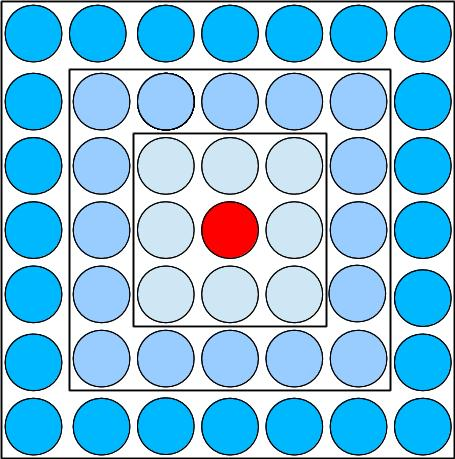
\includegraphics[width=0.3\linewidth]{img/parte2-vecindario.jpg}
	\caption{Función de vecindario.}
	\label{vecindario}
\end{figure}

Esta topología esta definida como la distacia euclidiana. 

\begin{algorithm}
	\caption{ddistance(self, i, j):}
	\begin{algorithmic}
		\State $w = self._output_layout[0]$
		\State $h = self._output_layout[1]$
		\State $min_x = min(i[0], j[0])$
		\State $min_y = min(i[1], j[1])$
		\State $max_x = max(i[0], j[0])$
		\State $max_y = max(i[1], j[1])$

		\State $dist_x = min(max_x-min_x, min_x + w - max_x)$
		\State $dist_y = min(max_y - min_y, min_y + h - max_y)$

		\State return $math.sqrt(dist_x**2 + dist_y**2)$
	\end{algorithmic}
\end{algorithm}

Este algoritmo tiene la característica particular de ser toroidal por lo cual la superficie de revolución generada por el plano gira alrededor de un eje tal como se muestra en la Fig~\ref{dist-euclideana}.

\begin{figure}[ht!]
	\centering
	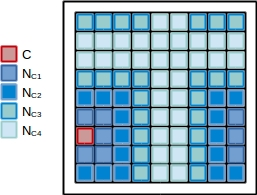
\includegraphics[width=0.5\linewidth]{img/parte2-toroidal.jpg}
	\caption{Distancia euclidiana toroidal}
	\label{dist-euclideana}
\end{figure}

En la figura anterior se puede ver que dada una neurona ganadora $c$, se definen $N_{c1}$, $N_{c2}$, $N_{c3}$, $N_{c4}$ como las neuronas vecinas, siendo, $N_{c1}$ las vecinas inmediatas y $N_{c4}$ las vecinas más lejanas a $c$. Este tipo de topología fuerza a que los pesos no crezcan en forma desmedida con respecto a las neuronas vecinas. Dichos pesos los actualizamos mediante la Regla de Kohonen:

\begin{align*}
	W_{i}(t+1) &=  \begin{cases}
						W_{i}(t) + \alpha(t) [ \varepsilon(t) - W_{i}(t) ] & i \in N_{c} \\
						W_{i}(t)                                           & i \not \in N_{c}  
					\end{cases} \\
\end{align*}

Para que un modelo sea auto-organizado debemos elegir el sigma $\sigma$ y  el eta $\eta$ adecuados. El $\sigma$ será utilizado como parámetro de la Gauseana y medirá la dispersión, cuántas neuronas vecinas a la neurona activada modificarán sus pesos. Por otro lado, el $\eta$ será el coeficiente de aprendizaje de nuestra red. 
Inicialmente el vecindario está definido como todas las neuronas del plano, pero con el correr del tiempo 
este vecindario disminuye su tamaño hasta afectar solamente el peso de la neurona ganadora. En un principio estos valores los habiamos inicializado muy grandes porque lo que nuestra red nunca se ordenaba, por lo que  fuimos variándolos hasta que llegamos a los óptimos. Si estos coeficientes eran siempre los mismos con el correr del tiempo, no llegabamos a ordenar la red, por lo que optamos por hacerlos dinámicos. 
Para hacer $\sigma$ dinámico utilizamos la siguiente función:
\begin{align*}
		\sigma(t) = \frac{\sigma_{0}}{1 + t \sigma_{0} \sigma_{r}} 
\end{align*}

$\sigma_{r}$ está definido como $0.005$ y $\sigma_{0}$ es:

\begin{align*}
		\sigma_{0} = 4.5 * \frac{outputlayout[0]}{10} 
\end{align*}

Para definir estos valores nos basamos en valores experimentales:

\begin{itemize}
	\item $\sigma_{0}$: En un principio lo habíamos inicializado en 1 pero esto hacía que el vecindario sea muy angosto por lo que nunca llegaba a organizarse ya que los vecimos de una neurona ganadora eran relativamente pocos y esto hacía lo que rápidamente el vecindario se achicaba hasta afectar solo a la neurona ganadora. Por ende el mapa quedaba desorganizado. Esto lo solucionamos agrandando el $\sigma_{0}$ para que cubra todo el mapa y con esto se organizó bien.
	\item $\sigma_{r}$: Fuimos probando con distintos valores hasta conseguir que el tamaño del vecindario no descendiera ni muy rápido ni muy despacio, encontrando que el mejor valor era $0.005$. 
\end{itemize}	

Para colorear el layout utilizamos el siguiente criterio: A cada categoría le asignamos un color. Para cada unidad de entrada contamos los inputs que están asociados a la misma categoría y de ellos elegimos la categoría que corresponda a la mayoría. Uno de los problemas que no solucionamos fue cuando los porcentajes de categorías son similares. Por ejemplo: Dadas las categorías A, B y C. Si a una neurona le corresponde en un 40$\%$ la Categoría A, 40$\%$ la Categoría B y 20$\%$ la Categoría C nuestro algoritmo no es del todo confiable.

El layout es un plano en el que coloreamos las coordenadas del color asociado a la categoría de la neurona ganadora. Este puede tener distintas dimensiones según lo definamos. Nosotros elegimos que nuestro layout tenga dimensión 15 $x$ 15 y un ejemplo de coloreo es la Fig~\ref{ejemplo}.

\begin{figure}[ht!]
	\centering
	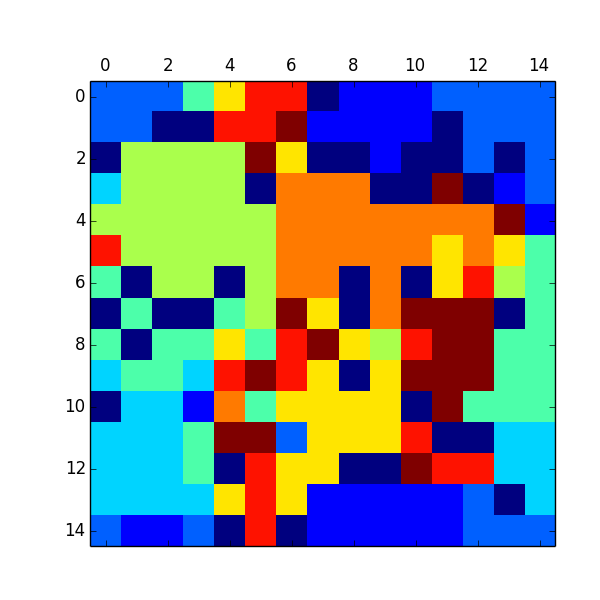
\includegraphics[width=0.7\linewidth]{img/parte2-ejemplocoloreo.png}
	\caption{Ejemplo de Layout de dimensión 15x15.}
	\label{ejemplo}
\end{figure}

Para el clasificador del conjunto de test, dado un X buscamos la unidad que más se parece a $X$ en $W$ y asignamos la categoría de la misma, como señala la Fig~\ref{comparacion} y da como resultado, por ejemplo, la Fig~\ref{ejemplo}. En este clasificador no consideramos las unidades a las que el training no les asignó categoría. En la Fig~\ref{ejemplo} se puede ver como se clasificó según las distintas categorías, pero algunas no fueron clasificadas, como por ejemplo las de color azul. Esto se debe a que ... \textbf{COMPLETAR!!!}

\subsection{Ejecución}

\subsubsection{Modo de uso}

\textbf{Para entrenar la red:}

\begin{lstlisting}[style=bash]
usage: khtrain.py [-h] -p P -x X -w W -l L -n N

Parametros de la red

optional arguments:

  -h, --help  show this help message and exit

  -p P        Ruta del archivo de salida para escribir pesos

  -x X        Archivo de training features

  -w W        Ancho del arreglo de neuronas de salida

  -l L        Alto del arreglo de neuronas de salida

  -n N        Cantidad de epochs a entrenar
\end{lstlisting}

Ejemplo: 

\noindent\texttt{python khtrain.py -x <el archivo con los datos de train> -p <el archivo de salida con los pesos> -w 15 -l 15 -n <epochs>} \\

\textbf{Para mostrar el mapa coloreado según las categorías:}

\begin{lstlisting}[style=bash]
usage: khdispplaymap.py [-h] -p P

Parametros

optional arguments:

  -h, --help  show this help message and exit

  -p P        Ruta del archivo de entrada con los pesos para mostrar el mapa

\end{lstlisting}

Ejemplo:

\noindent\texttt{python khdispplaymap.py -h} \\


\textbf{Para el clasificador:}

\begin{lstlisting}[style=bash]
usage: khclassify.py [-h] -p P -x X

Parametros de la red

optional arguments:

  -h, --help  show this help message and exit

  -p P        Ruta del archivo de entrada con los pesos

  -x X        Archivo de features
\end{lstlisting}

Ejemplo:

\noindent\texttt{python khclassify.py -h} \\

\begin{figure}[ht!]
	\centering
	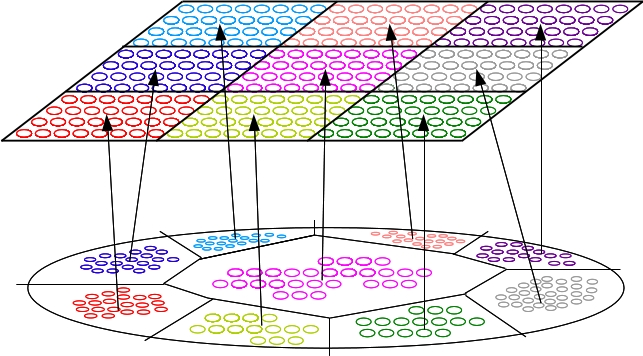
\includegraphics[width=0.8\linewidth]{img/parte2-kohonen9clases.jpg}
	\caption{Clasificación con Kohonen}
	\label{Kohonen}
\end{figure}


\subsection{Resultados}
Como resultados importantes podemos decir que llegamos a un orden de predicción de clasificación del 80$\%$, lo cual nos parece bastante bueno considerando que eran pocos datos de entrenamiento y que los datos del dataset no eran totalmente separables.

\subsection{Conclusiones}
Como conclusiones podemos mencionar que la tarea de encontrar valores óptimos de $\eta$, $\sigma_{0}$, $\sigma_{r}$ fue bastante difícil, ya que si los valores no eran los correctos, ya sean muy grandes o muy chicos, la red no se organizaba.
Por otro lado, nos parece un algoritmo lento ya que por cada iteración se recorre cada ejemplo contra todas las neuronas lo que produce que dé como resultado un orden de complejidad bastante elevado para que converja nuestro algoritmo.